\documentclass[11pt]{article}

% =========================================================================
% document style changes
% =========================================================================

\usepackage{amsmath}                    % AMS math packages
\usepackage{amssymb}                    %
\usepackage[]{graphpap}
\usepackage[T1]{fontenc}                % for \mathrm{}
\usepackage{courier}                    % for \texttt{}
\usepackage{bbm}                        % for \mathbbm{1} (indicator function)
\usepackage{booktabs}
\usepackage{graphicx}
\usepackage[font={small}]{caption}
\usepackage{subcaption}

%\setlength{\parskip}{\baselineskip}     % skip line following paragraphs
%\pagestyle{empty}                       % No page numbers
\setlength{\topmargin}{-.5in}
\setlength{\textheight}{9in}
\setlength{\oddsidemargin}{.125in}
\setlength{\textwidth}{6.25in}

\newcommand{\spc}{\vspace{0.25in}}      % Shortcut commands
\newcommand{\ds}{\displaystyle}         %\newcommand{\ds}[1]{\displaystyle{#1}}
\newcommand{\ra}{\rightarrow}
\DeclareMathOperator*{\argmax}{arg\!\max}
\DeclareMathOperator*{\argmin}{arg\!\min}

\begin{document}                        % This is where the document begins

\title{Improving Item-Item Similarity Estimation during Collaborative Filtering}
\author{Bill Chickering and Jamie Irvine\\
CS 399 with Anand Rajaraman\\
Stanford University}
\renewcommand{\today}{March 25, 2014}
\maketitle

\section*{Abstract}
\emph{Will write this when the paper is done}

\section*{Introduction}
The similarity of two items is a valuable measurement for a number of
data-mining applications, such as recommender systems. With large amounts of
rating data, collaborative filtering is a good method for calculating
similarity. However, with sparse rating data, this technique gives noisy and
unreliable approximations for similarity. Even worse, low confidence
measurements of similarity are indistinguishable from high confidence ones. In
this paper, we develop and compare a number of methods to produce more accurate
estimates of similarity by incorporating confidence into the similarity score.
 
Item-based collaborative filtering is a common technique for measuring the
similarity of two items. There are different forms of collaborative filtering.
For this paper, we use a traditional approach. Each item is represented as a
vector of ratings. The similarity score of two items is computed by measuring
the similarity of the two rating vectors.

There are a few ways to compute the similarity of two vectors. One approach is
to use Cosine-similarity, defined as the cosine of the angle between the two
vectors:
\begin{align}
CosSim(A, B) = \frac{\sum\limits_{u\in U_{AB}}
r_{u,A}r_{u,B}}{\sqrt{\sum\limits_{u\in U_{A}} r_{u,A}^2}
\sqrt{\sum\limits_{u\in U_{B}} r_{u,B}^2}}
\end{align}
where $U_{I}$ is the set of all users who rated item $I$, $U_{AB}$ is the set of
all users who rated both item $A$ and item $B$ and $r_{u,I}$ is the rating user
$u$ gave to item $I$. Another popular approach is to use Pearson correlation:
\begin{align}
PearsSim(A, B) = \frac{\sum\limits_{u\in U_{AB}}
r_{u,A}r_{u,B}}{\sqrt{\sum\limits_{u\in U_{AB}} r_{u,A}^2}
\sqrt{\sum\limits_{u\in U_{AB}} r_{u,B}^2}}
\end{align}

Other similarity functions exist, such as one-sided similarities, but Pearson
correlation and Cosine-similarity are the most popular and will be the two
measurements used in this paper. \footnotemark

\footnotetext{ Note that the difference between the two similarities is how they
handle unpaired ratings; that is ratings from a user who has not rated the other
item. Cosine-similarity considers the unknown rating from an unpaired rating to
be $0$ and then calculates the cosine of the two vectors. Pearson correlation
simply throws away all unpaired ratings and calculates the cosine of the two
modified vectors.}

Both similarity measurements primarily leverage information from common users,
that is users who have rated both items. Because of this, they perform well with
a large number common users, but give unreliable results when the items have few
common users. In an extreme case, if only one user has rated item $A$ and item
$B$, $PearsSim(A, B) = 1$ or $-1$. Not only is this unlikely to be an accurate
assessment of the true similarity of $A$ and $B$, it also gives the most extreme
results possible, without giving any indication that this is a low-confidence
calculation.

In this paper, we construct a more accurate similarity score by incorporating
the number of common users, $n$, into the similarity function. 

\section*{Problem}

The goal is to calculate a modified similiary function that leverages the number
of commonn users to better estimate the true similarity. Formally, we design
$ModSim$ such that for two items $A$ and $B$ with $n$ users in common

\begin{align}
ModSim(A, B, n) \approx TrueSim(A, B)
\end{align}
where $TrueSim$ is the true similarity of the two items. Of course, there is no
way to actually know the true similarity of two items, but for a good enough
similarity function, such as $PearsSim$ or $CosSim$ and a large enough $n$, we
can get a good estimate. Thus, we model $TrueSim$ as 
\begin{align}
TrueSim(A, B) = lim_{n\to\infty}Sim(A, B)
\end{align}
where $Sim$ is the most appropriate generic similarity function for the dataset.

Since $TrueSim$ dependends on the choice of $Sim$, we abstract away the details
of $Sim$ and use its output directly. In all, the goal is to construct $ModSim$
such that

\begin{align}
ModSim(Sim(A, B), n) \approx lim_{n\to\infty}Sim(A, B)
\end{align}

\section*{Model}

We model the problem probabilistically. Let $Y$ be a random variable
representing the $TrueSim$ of a randomly chosen pair of items. Let $X_n$ be a
random variable representing the calculated $Sim$ of a pair of items with $n$
common users.

We model $Y$ as a Normal distribution 
\begin{align}
Y \sim N(\mu, \sigma_{1}^2)
\end{align}
where $\mu$ and $\sigma_{1}^2$ are the average similarity score and the variance
of similarity scores of all pairs of items, respectively. Since $X_n$ represents
a noisy reading of the true similarity $Y$, we model $X_n | Y$ as a Gaussian
error around $Y$:
\begin{align}
(X_n | Y=y) \sim N(y, \sigma_{2, n}^2)
\end{align}

Note that $\sigma_{2, n}^2$ represents how noisy the estimation of $Sim$ is when
there are $n$ common users. This should decrease as $n$ increases.

\begin{figure}[!htbp]
    \centering
    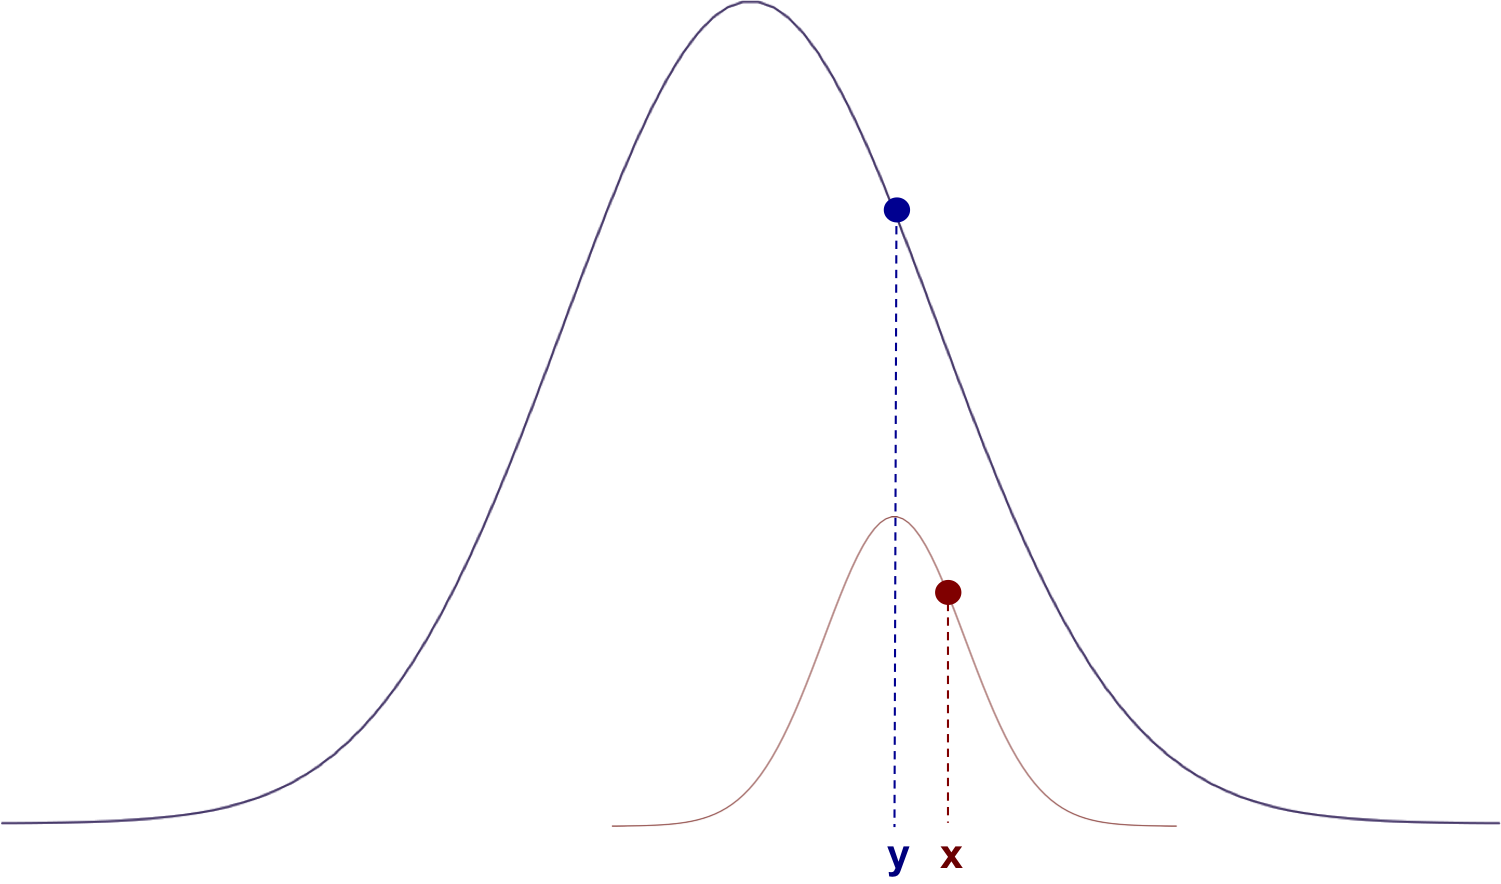
\includegraphics[width=0.5\textwidth]{twonormals.png}
	\caption{The blue curve represents $Y$, the distribution of true
    similarities between a random pair of items. The red curve represents $X|Y$,
    the observed similarity when a small number of common users exist.}
    \label{fig:two_normals}
\end{figure}

In probabilistic terms, for a calculated value $X_n$, we want to find the value
of $Y$ that most likely produced $X_n$. Thus we desire the Maximum Likelihood
Estimate of $Y | X_n$
\begin{align}
\argmax_yP(Y=y|X_n=x) &= \argmax_y\left[\frac{P(X_n=x |
Y=y)P(Y=y)}{P(X_n=x)}\right]
\\&= \argmax_y\left[P(X_n=x|Y=y)P(Y=y)\right]
\\&= 
\argmax_y\left[\frac{1}{\sigma_{2,n}\sqrt{2\pi}}\exp{\left(\frac{-(x-y)^2}
{2\sigma_{2,n}^2}\right)}
\frac{1}{\sigma_{1}\sqrt{2\pi}}\exp{\left(\frac{-(y-\mu)^2}
{2\sigma_{1}^2}\right)}\right]
\\&= \argmin_y\left[\frac{(x-y)^2}{2\sigma_{2,n}^2} +
\frac{(y-\mu)^2}{2\sigma_{1}^2}\right]
\\&= \argmin_y\left[\left(\sigma_{1}^2+\sigma_{2,n}^2\right)y^2 - 
2\left(\sigma_{1}^2x+\sigma_{2,n}^2\mu\right)y\right]
\end{align}
We find the exact minimum by taking the derivative with respect to $y$ and
setting it to zero:
\begin{align}
\frac{d}{dy}\left[\left(\sigma_{1}^2+\sigma_{2,n}^2\right)y^2 - 
2\left(\sigma_{1}^2x+\sigma_{2,n}^2\mu\right)y\right]
&= 2\left(\sigma_{1}^2+\sigma_{2,n}^2\right)y - 
2\left(\sigma_{1}^2x+\sigma_{2,n}^2\mu\right) 
\\&= 0
\end{align}
Solving for y:
\begin{align}
y &= \frac{\sigma_{1}^2x+\sigma_{2,n}^2\mu}{\sigma_{1}^2+\sigma_{2,n}^2}
\end{align}
which can be rewritten as:
\begin{align}
\left(y - \mu\right) &= \frac{\sigma_{1}^2}{\sigma_{1}^2+\sigma_{2,n}^2}
\left(x-\mu\right)
\end{align}

The model suggests that there is a linear correlation between $X_n$, the
similarity calculated with $n$ common users, and $Y$, the true similarity.
Moreover, the best predicted $y$ is a linear combination of the mean and the
observed similiatiry. Since $\sigma_{2,n}^2\ge0$, the slope is always $\le1$, 
meaning that the calculated distance from $\mu$ (the average similarity) 
overestimates the true distance. This makes sense, since there is a prior 
distribution of true similarity weighted around $\mu$.

The parameters $\mu$, $\sigma_{1}^2$, and $\sigma_{2,n}^2$ all can be approximated 
using the method of moments over training data where there are enough common
users that $TrueSim$ can be approximated. This method requires approximating
$\sigma_{2,n}^2$ for every value of $n$ separately. Alternatively, we can model
$\sigma_{2,n}^2$ as a function of $n$. Recall that $\sigma_{2,n}^2$ is the
noisiness of the measurement $Sim$ about $TrueSim$ and $TrueSim = lim_{n \to
\infty}Sim$. Thus $Sim$ can be thought of as a sampling $n$ users from the
infinite set used to calculate $TrueSim$. Although $Sim$ may not be linear, we
the Central Limit Theorem motivates the intuition that the variance of $Sim$
would decrease as the $sqrt(n)$. Thus we model $\sigma_{2,n}^2$ as:
\begin{align}
\sigma_{2,n}^2 = \frac{\alpha}{\sqrt{n}},
\end{align}
yielding the single parameter model:
\begin{align}
\left(Y - \mu\right) = \frac{\sigma_{1}^2}{\sigma_{1}^2+\frac{\alpha}{\sqrt{n}}}
\left(X_n-\mu\right)
\end{align}
In terms of a modified similarity function, as desired earlier, we now have:
\begin{align}
ModSim(Sim, n) = \frac{\sigma_{1}^2}{\sigma_{1}^2+\frac{\alpha}{\sqrt{n}}}
\left(Sim-\mu\right) + \mu
\end{align}

\section*{Technique}
Based on this maodel, we try three different techniques to predict the true similarity from a
measured similarity. The techniques vary in their fidelity to the model. For
each, we limit our data to all pairs of items that have enough common users that
we can approximate $TrueSim \approx Sim$. Then we pick subsets of the common
users of various sizes $n$ and calculate $Sim_{n}$. With examples of $Sim$, $n$
and the resulting $TrueSim$, we can implement supervised learning.

The first technique is the least faithful to the model. It simply runs a number
of linear regressions between $Sim$ and $TrueSim$ for each $n$. This ignores the 
data-specific parameters $\mu$, $\sigma_{1}$ and $\sigma_{2,n}$ to find the best 
linear fit. It also treats each $n$ completely independently. This technique 
necessarilty has the lowest training error of all linear techniques, potentially 
at the risk of overfitting.

The second technique is more general. It approximates $\mu$ and $\sigma_{1}$
using the method of moments on the training data of all $TrueSim$ scores. Then,
$\sigma_{2,n}$ is also approximated using a method of moments on the training
data of all $Sim_n$ for each $n$ separately. Here $\sigma_{2,n}$'s are also
considered independently of each other.

The third and most general technique models $\sigma_{2,n}$ as a function of
$n$ using equation 19. As in the previous technique, $\mu$, $\sigma_{1}$ and each
$\sigma_{2,n}$ are approximated using the method of moments over the training
data. Then $\alpha$ is calculated that minimizes the sum of squared errors
between $\sigma_{2,n}^2$ and $\frac{\alpha}{\sqrt{n}}$. This $\alpha$ is used to
construct the three-parameter prediction function of equation 19.

\section*{Experiment}

\section*{Results}

\begin{figure}[!htbp]
    \centering
    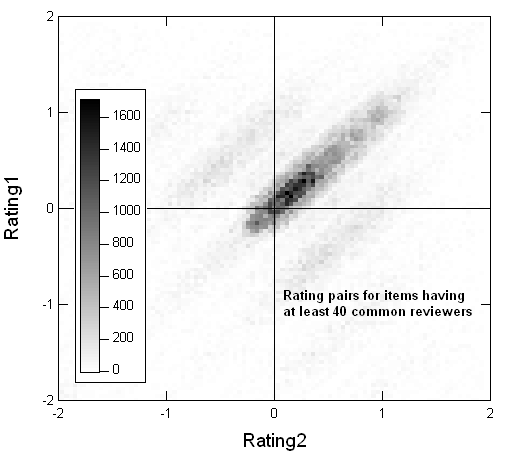
\includegraphics[width=0.7\textwidth]{RatingDist_40.png}
    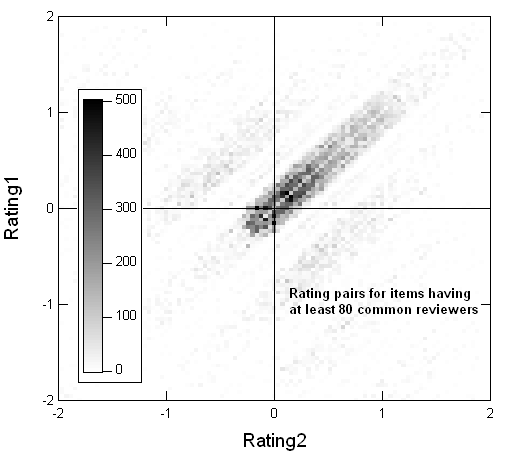
\includegraphics[width=0.7\textwidth]{RatingDist_80.png}
	\caption{Distribution of rating pairs by common reviewers for item pairs.
Top figure shows distribution for item pairs having at least 40 common
reviewers. Bottom figure shows distribution for item pairs having at least 80
common reviewers.}
    \label{fig:RatingDist}
\end{figure}

\begin{figure}[!htbp]
    \centering
    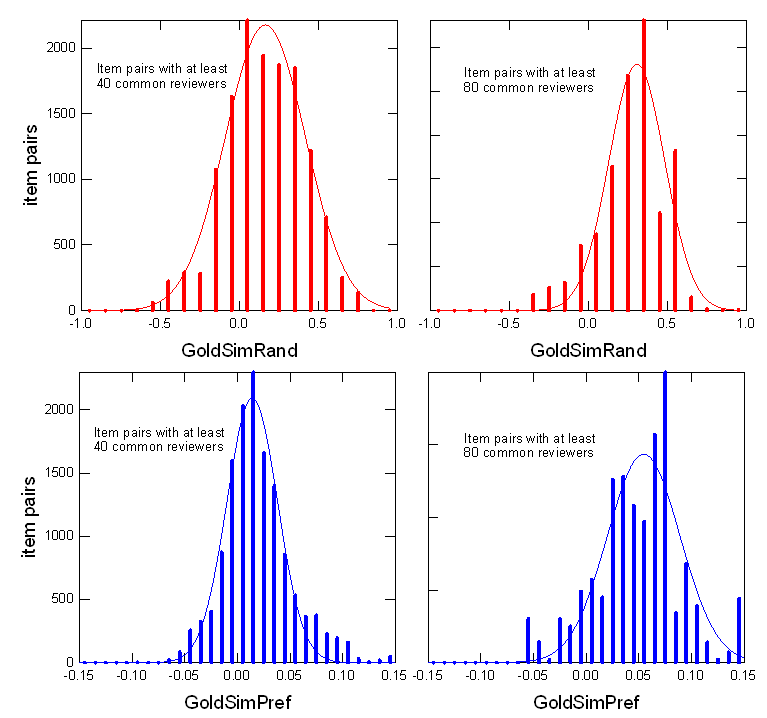
\includegraphics[width=1.0\textwidth]{Histograms.png}
	\caption{Histograms of {\em TrueSimR} (top) and {\em TrueSimP} (bottom) for
training datasets containing at least 40 common reviewers (left) and 80 common
reviewers (right).}
    \label{fig:Histograms}
\end{figure}

\begin{figure}[!htbp]
    \centering
    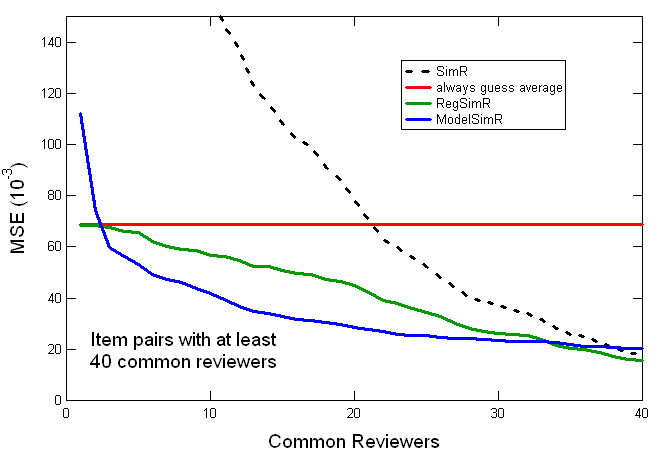
\includegraphics[width=0.9\textwidth]{MSE_SimR_40.png}
    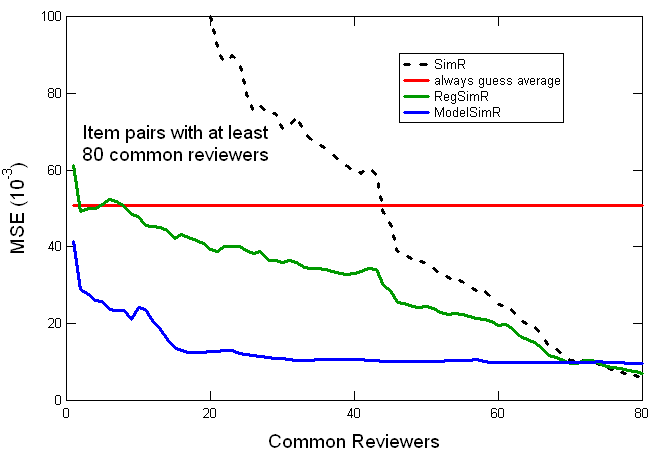
\includegraphics[width=0.9\textwidth]{MSE_SimR_80.png}
	\caption{Mean square error {\em vs} number of common reviewers, $n$, for
estimates of {\em TrueSimR} for item pairs ultimately having at least 40 common
reviewers (top) and 80 common reviewers (bottom). The dashed curve represents
{\em SimR} computed using only the ratings from the first $n$ reviewers. The
flat red line indicate the MSE that results from always guessing the average
{\em TrueSimR} from the training set. The green curve is {\em RegSimR} and the
blue curve is {\em ModelSimR}. }
    \label{fig:MSE_SimR}
\end{figure}

\begin{figure}[!htbp]
    \centering
    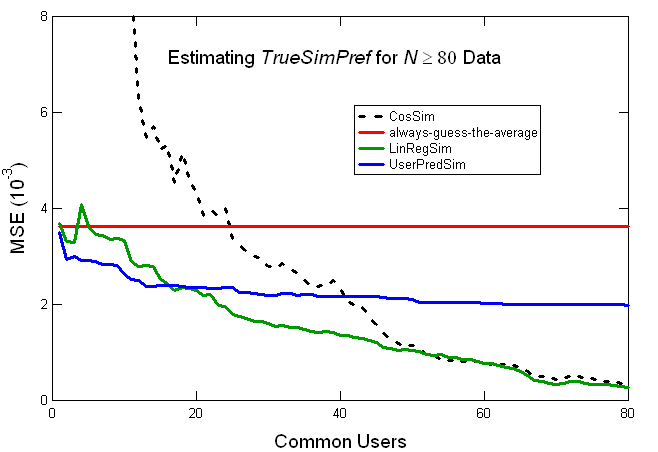
\includegraphics[width=0.9\textwidth]{MSE_SimP_80.png}
	\caption{Mean square error {\em vs} number of common reviewers, $n$, for
estimates of {\em TrueSimP} for item pairs ultimately having at least 80 common
reviewers. The dashed curve represents
{\em SimP} computed using only the ratings from the first $n$ reviewers. The
flat red line indicate the MSE that results from always guessing the average
{\em TrueSimP} from the training set. The green curve is {\em RegSimP} and the
blue curve is {\em ModelSimP}. }
    \label{fig:MSE_SimP}
\end{figure}

\section*{Conclusion}

\end{document}
